\documentclass[11pt,letterpaper]{article}

\usepackage[utf8]{inputenc}
\usepackage[T1]{fontenc}
\usepackage[brazil]{babel}
\usepackage{lmodern}
\usepackage{geometry}
\usepackage{graphicx}
\usepackage{amsmath,amssymb}
\usepackage{booktabs}
\usepackage{array}
\usepackage{float}
\usepackage{subcaption}
\usepackage{xcolor}
\usepackage{hyperref}
\usepackage{microtype}
\usepackage{fancyhdr}
\usepackage{listings}

\geometry{top=2.25cm,bottom=2.25cm,left=2.45cm,right=2.45cm}
\graphicspath{{figures_tc02/}}
\definecolor{reportblue}{HTML}{2F5D7C}
\definecolor{lightblue}{HTML}{DCE9F1}
\hypersetup{
  colorlinks=true,
  linkcolor=reportblue,
  urlcolor=reportblue,
  citecolor=reportblue,
  pdftitle={Alto-falante eletrodinâmico -- Trabalho Computacional 02},
  pdfauthor={Matheus Carvalho; Talvani de Souza; Gustavo Augusto Ortiz; Gabriel de Araújo}
}
\setlength{\parindent}{1.25cm}
\setlength{\parskip}{0.15em}
\renewcommand{\arraystretch}{1.18}
\pagestyle{fancy}
\fancyhf{}
\fancyhead[L]{\small EEE050 -- Modelagem e Simulação Multifísica}
\fancyhead[R]{\small Trabalho Computacional 02}
\fancyfoot[C]{\thepage}
\setlength{\headheight}{14pt}
\lstset{
  language=Python,
  basicstyle=\ttfamily\small,
  keywordstyle=\color{reportblue}\bfseries,
  commentstyle=\color{gray},
  stringstyle=\color{reportblue},
  frame=single,
  rulecolor=\color{lightblue},
  breaklines=true,
  showstringspaces=false,
  columns=fullflexible
}

\begin{document}

\hypersetup{pageanchor=false}
\begin{titlepage}
  \thispagestyle{empty}
  \centering
  {\color{reportblue}\rule{0.82\textwidth}{1.2pt}}\\[1.3cm]
  {\large\bfseries EEE050}\\[0.35cm]
  {\large Modelagem e Simulação Multifísica}\\[0.25cm]
  {\normalsize Engenharia de Sistemas -- 2026/02}\\[1.25cm]
  {\color{lightblue}\rule{0.82\textwidth}{5pt}}\\[1.15cm]
  {\color{reportblue}\fontsize{23}{28}\selectfont\bfseries ALTO-FALANTE ELETRODINÂMICO}\\[0.45cm]
  {\large Relatório do Trabalho Computacional 02}\\[1.0cm]
  {\color{lightblue}\rule{0.82\textwidth}{5pt}}\\[1.35cm]
  {\large\bfseries Autores}\\[0.55cm]
  {\large
    Gabriel de Araújo\\
    Gustavo Augusto Ortiz\\
    Matheus Carvalho\\
    Talvani de Souza
  }\\[1.5cm]
  \vfill
  {\large 30 de agosto de 2026}\\[0.75cm]
  {\color{reportblue}\rule{0.82\textwidth}{1.2pt}}
\end{titlepage}

\hypersetup{pageanchor=true}
\pagenumbering{arabic}
\setcounter{page}{1}
\tableofcontents
\clearpage

\section{Introdução}

O presente relatório documenta o segundo trabalho computacional da disciplina de Modelagem e
Simulação Multifísica. O objeto de estudo é um alto-falante eletrodinâmico, sistema no qual uma
tensão aplicada à bobina produz corrente elétrica e força magnética; essa força movimenta o conjunto
móvel formado pela bobina e pelo cone, gerando uma onda acústica. O dispositivo reúne, portanto,
fenômenos eletromagnéticos, elastodinâmicos e acústicos acoplados.

O trabalho tem quatro objetivos principais: simular o modelo linear com uma gravação de voz;
comparar a entrada elétrica com a aceleração do cone nos domínios do tempo e da frequência;
introduzir uma dependência não linear do fator de força $Bl$ com o deslocamento; e comparar os
modelos linear e não linear quando excitados por uma senoide dentro da faixa da voz humana. As
simulações foram implementadas em Python no arquivo \texttt{TC2.ipynb}, empregando integração
numérica de problemas de valor inicial e a transformada discreta de Fourier.

\subsection{Descrição física do alto-falante}

O alto-falante considerado é composto por um ímã permanente, uma bobina móvel, elementos de
suspensão e um cone aproximadamente rígido. A corrente da bobina interage com o campo magnético
do ímã e produz a força de Laplace. A aranha e o anel de suspensão mantêm o alinhamento do
conjunto e oferecem uma força restauradora, enquanto o movimento do cone no ar introduz
amortecimento e gera pressão acústica.

\begin{figure}[H]
  \centering
  \begin{subfigure}[b]{0.34\textwidth}
    \centering
    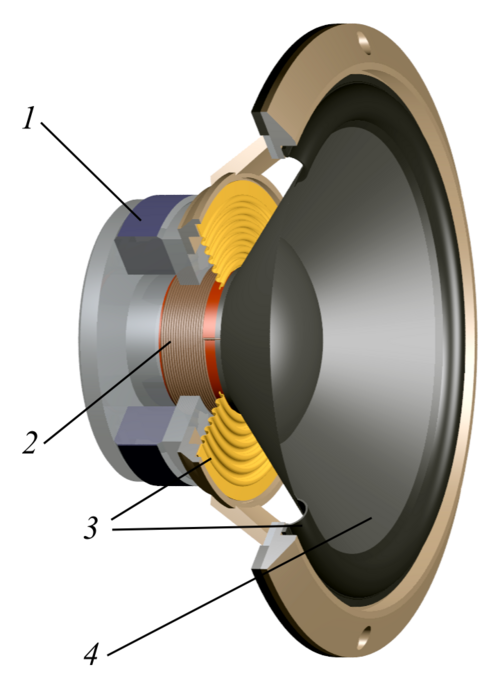
\includegraphics[height=4.4cm]{Loudspeaker-bass.png}
    \caption{Geometria externa.}
  \end{subfigure}\hfill
  \begin{subfigure}[b]{0.61\textwidth}
    \centering
    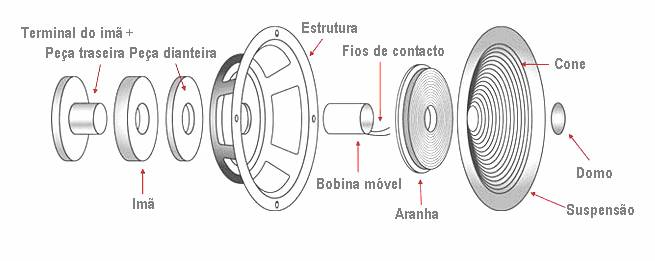
\includegraphics[width=\textwidth]{Aula04_alto-falante_partes.jpg}
    \caption{Principais componentes.}
  \end{subfigure}
  \caption{Representações do alto-falante eletrodinâmico utilizadas na contextualização do problema.}
  \label{fig:altofalante}
\end{figure}

Em uma descrição distribuída, a deformação das partes móveis é regida pelo equilíbrio do momento
linear, as grandezas elétricas e magnéticas obedecem às equações de Maxwell e a propagação sonora
é descrita pela equação de onda. Para a faixa de operação estudada, essas físicas são condensadas
em um modelo de parâmetros concentrados, adequado à simulação por equações diferenciais
ordinárias.

\subsection{Parâmetros e sinais de entrada}

Os parâmetros adotados são aqueles propostos no enunciado e empregados no notebook. As condições
iniciais de corrente, deslocamento e velocidade são nulas.

\begin{table}[H]
  \centering
  \caption{Parâmetros do modelo concentrado do alto-falante.}
  \label{tab:parametros}
  \begin{tabular}{clrl}
    \toprule
    Símbolo & Grandeza & Valor & Unidade \\
    \midrule
    $m$  & Massa do conjunto móvel       & $14{,}35\times10^{-3}$ & kg \\
    $b$  & Coeficiente de amortecimento  & $0{,}786$               & kg/s \\
    $k$  & Rigidez equivalente           & $1852$                  & N/m \\
    $Bl$ & Fator de força linear         & $4{,}95$                & N/A \\
    $L$  & Indutância da bobina          & $266\times10^{-6}$      & H \\
    $R$  & Resistência da bobina         & $3{,}3$                 & $\Omega$ \\
    \bottomrule
  \end{tabular}
\end{table}

A primeira entrada é uma gravação de voz estéreo com frequência de amostragem de
$44{,}1\,\mathrm{kHz}$ e duração de $9{,}61\,\mathrm{s}$. Os dois canais foram convertidos para mono
pela média aritmética e o resultado foi normalizado para amplitude máxima unitária, respeitando a
hipótese de tensão compatível com uma saída de áudio de computador. A segunda entrada é uma
senoide de $500\,\mathrm{Hz}$, amplitude de $2\,\mathrm{V}$ e duração igual à da gravação.

\section{Modelagem matemática}

\subsection{Modelo elétrico}

Do ponto de vista dos terminais, a bobina é representada por uma resistência $R$, uma indutância
$L$ e uma força contraeletromotriz proporcional à velocidade. Desprezando perdas magnéticas no
núcleo e aplicando a lei das tensões de Kirchhoff, obtém-se
\begin{equation}
  u(t)=Ri(t)+L\frac{di(t)}{dt}+Bl\frac{dx(t)}{dt},
  \label{eq:eletrica}
\end{equation}
em que $u(t)$ é a tensão aplicada, $i(t)$ é a corrente da bobina e $x(t)$ é o deslocamento axial do
cone. O termo $Bl\dot{x}$ representa a tensão induzida pelo movimento da bobina no campo
magnético e realiza o acoplamento da dinâmica mecânica com a elétrica.

\subsection{Modelo mecânico}

O conjunto móvel é aproximado por um sistema massa--mola--amortecedor. A força magnética é
$f_m=Bl\,i$, a força restauradora é $f_r=-kx$ e a força de amortecimento viscoso é
$f_a=-b\dot{x}$. Pela segunda lei de Newton,
\begin{equation}
  m\ddot{x}(t)=Bl\,i(t)-b\dot{x}(t)-kx(t).
  \label{eq:mecanica}
\end{equation}
Esse modelo assume movimento axial, cone rígido, parâmetros mecânicos constantes e ausência de
efeitos como modos de ruptura, histerese e dependência térmica da resistência.

\subsection{Representação em espaço de estados}

Definindo o vetor de estados $\boldsymbol{z}(t)=[i(t)\;x(t)\;v(t)]^{T}$, com
$v(t)=\dot{x}(t)$, as Equações~\eqref{eq:eletrica} e \eqref{eq:mecanica} resultam em
\begin{equation}
  \begin{aligned}
    \dot{i} &= -\frac{R}{L}i-\frac{Bl}{L}v+\frac{1}{L}u,\\
    \dot{x} &= v,\\
    \dot{v} &= \frac{Bl}{m}i-\frac{k}{m}x-\frac{b}{m}v.
  \end{aligned}
  \label{eq:estados}
\end{equation}
Na forma matricial,
\begin{equation}
  \dot{\boldsymbol{z}}=
  \underbrace{\begin{bmatrix}
    -R/L & 0 & -Bl/L\\
    0 & 0 & 1\\
    Bl/m & -k/m & -b/m
  \end{bmatrix}}_{\boldsymbol{A}}\boldsymbol{z}
  +
  \underbrace{\begin{bmatrix}1/L\\0\\0\end{bmatrix}}_{\boldsymbol{B}}u.
  \label{eq:matricial}
\end{equation}

A pressão acústica em um ponto de observação é, sob as simplificações adotadas, proporcional à
aceleração do cone. Se a saída mecânica escolhida for a velocidade, sua função de transferência é
$G(j\omega)=\boldsymbol{C}(j\omega\boldsymbol{I}-\boldsymbol{A})^{-1}\boldsymbol{B}$, com
$\boldsymbol{C}=[0\;0\;1]$. Assim, a resposta associada à aceleração é proporcional a
$j\omega G(j\omega)$.

\section{Procedimento computacional}

A gravação foi lida com \texttt{scipy.io.wavfile}. Após a conversão para mono e a normalização,
o vetor de tempo foi construído a partir da frequência de amostragem. O sistema de equações de
estado foi integrado com \texttt{scipy.integrate.solve\_ivp}; como o integrador escolhe instantes
internos próprios, a tensão foi obtida em cada avaliação por interpolação linear com
\texttt{numpy.interp}. O estado inicial foi $\boldsymbol{z}(0)=[0\;0\;0]^T$.

A aceleração não foi integrada como um estado independente, mas reconstruída da equação mecânica:
\begin{equation}
  \ddot{x}(t)=\frac{Bl\,i(t)-b\,v(t)-k\,x(t)}{m}.
  \label{eq:aceleracao}
\end{equation}
Os espectros unilaterais foram calculados com a transformada rápida de Fourier real. Para permitir
comparações entre sinais com unidades diferentes, suas magnitudes espectrais foram normalizadas
pelo respectivo valor máximo. Por fim, a aceleração foi normalizada e convertida para PCM de
16 bits para a geração dos arquivos de áudio de saída.

\section{Atividade 1: modelo linear}

\subsection{Entrada nos domínios do tempo e da frequência}

A Figura~\ref{fig:entrada} apresenta a gravação utilizada como tensão de entrada. No domínio do
tempo observam-se blocos de fala separados por intervalos de menor energia. O espectro concentra
suas componentes mais intensas aproximadamente entre dezenas e centenas de hertz, como esperado
para voz, e decai nas frequências mais elevadas.

\begin{figure}[H]
  \centering
  \begin{subfigure}[t]{0.49\textwidth}
    \centering
    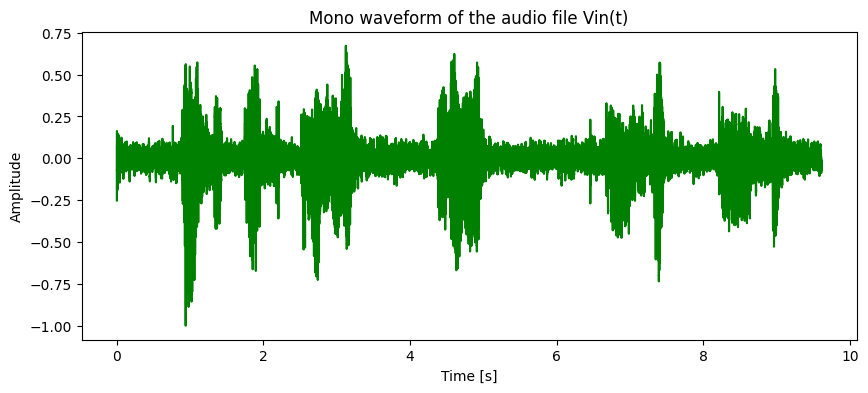
\includegraphics[width=\textwidth]{fig01_vin_time.png}
    \caption{Forma de onda de $V_{in}(t)$.}
  \end{subfigure}\hfill
  \begin{subfigure}[t]{0.49\textwidth}
    \centering
    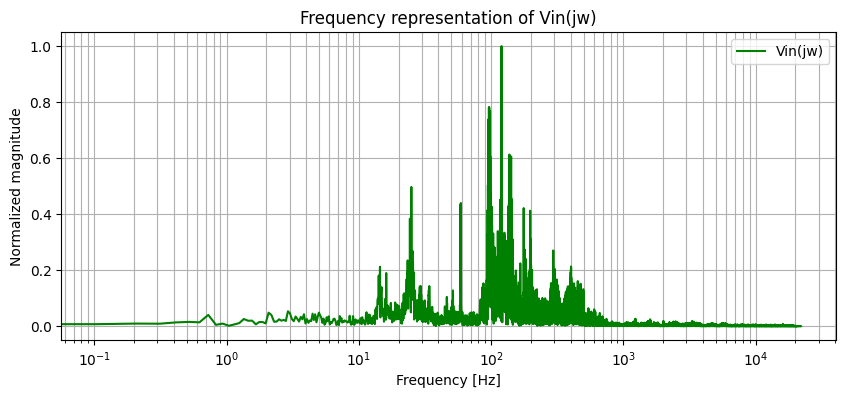
\includegraphics[width=\textwidth]{fig02_vin_freq.png}
    \caption{Magnitude normalizada de $V_{in}(j\omega)$.}
  \end{subfigure}
  \caption{Representações temporal e espectral da gravação de voz.}
  \label{fig:entrada}
\end{figure}

\subsection{Resposta temporal}

A resposta simulada do modelo linear é mostrada na Figura~\ref{fig:linear}. A corrente acompanha
a estrutura temporal da tensão e atinge aproximadamente $0{,}253\,\mathrm{A}$ em módulo. O
deslocamento máximo do cone é $0{,}121\,\mathrm{mm}$ e a aceleração chega a cerca de
$89{,}3\,\mathrm{m/s^2}$. Os três sinais permanecem limitados e retornam à vizinhança de zero nos
trechos sem excitação, resultado compatível com um sistema amortecido e estável.

\begin{figure}[H]
  \centering
  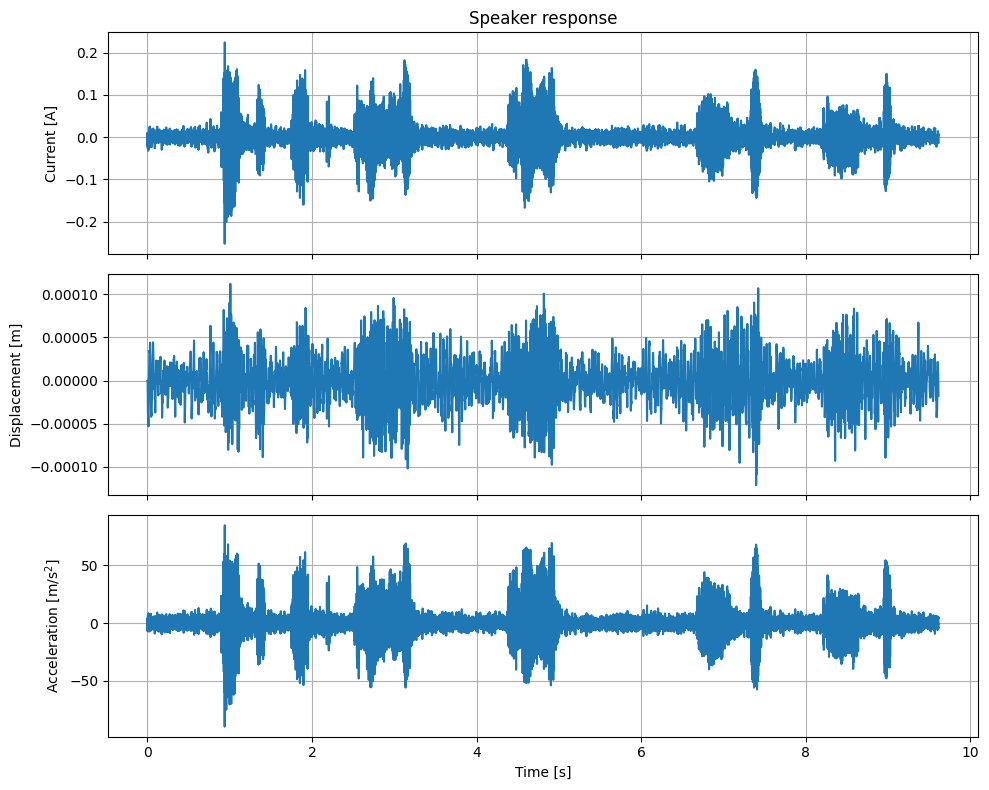
\includegraphics[width=0.88\textwidth]{fig03_linear_states.png}
  \caption{Corrente, deslocamento e aceleração do modelo linear para a gravação de voz.}
  \label{fig:linear}
\end{figure}

\subsection{Comparação entre entrada e aceleração}

A Figura~\ref{fig:comparacao-linear} permite comparar a entrada com a grandeza relacionada à
pressão acústica. A aceleração preserva a organização temporal da fala: os maiores eventos do sinal
de entrada produzem os maiores movimentos do cone. Contudo, sua forma de onda não é apenas uma
cópia amplificada de $V_{in}$, pois a combinação de inércia, rigidez, amortecimento e dinâmica
elétrica filtra o sinal.

No domínio da frequência, as componentes presentes em $V_{in}$ permanecem identificáveis na
aceleração, mas com ponderações diferentes. Em particular, componentes muito baixas são atenuadas
pela rigidez da suspensão, enquanto a passagem de velocidade para aceleração acrescenta um fator
proporcional à frequência. A interação desses efeitos determina a coloração espectral do áudio
reproduzido.

\begin{figure}[H]
  \centering
  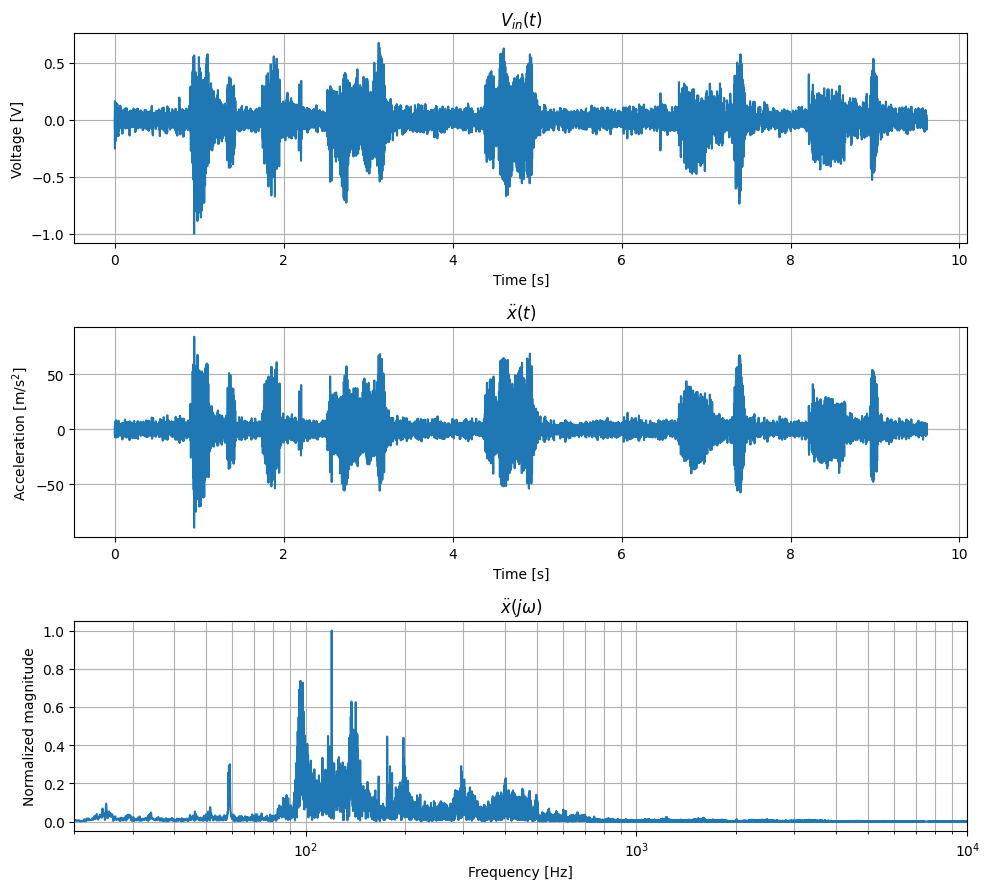
\includegraphics[width=0.86\textwidth]{fig04_linear_compare.png}
  \caption{Comparação temporal entre $V_{in}$ e $\ddot{x}$ e espectro normalizado da aceleração no modelo linear.}
  \label{fig:comparacao-linear}
\end{figure}

A aceleração normalizada foi salva como \texttt{TC02-out1.wav}. A normalização torna o arquivo
audível sem saturação digital, mas elimina a informação de amplitude física absoluta; por isso, a
avaliação quantitativa utiliza os valores anteriores à conversão para PCM.

\section{Atividades 2 e 3: modelo não linear}

\subsection{Definição do fator de força variável}

No modelo não linear, o fator de força diminui quando o cone se afasta da posição de repouso. A
excursão máxima do modelo linear, $x_{\max}=0{,}1214\,\mathrm{mm}$, define os limites
\begin{equation}
  x_1=0{,}75x_{\max}=0{,}0911\,\mathrm{mm},\qquad
  x_2=1{,}50x_{\max}=0{,}1821\,\mathrm{mm}.
  \label{eq:limites}
\end{equation}
A implementação quadrática utilizada no notebook é
\begin{equation}
Bl(x)=
\begin{cases}
Bl_0, & |x|\leq x_1,\\[2mm]
Bl_0\left(1-\dfrac{|x|-x_1}{x_2-x_1}\right)^2,
  & x_1<|x|<x_2,\\[3mm]
0, & |x|\geq x_2,
\end{cases}
\label{eq:bl-nl}
\end{equation}
com $Bl_0=4{,}95\,\mathrm{N/A}$. A expressão é contínua nos dois limites, mantém o modelo linear
para pequenas excursões e representa a perda de acoplamento eletromecânico nas excursões maiores.

Substituindo $Bl$ por $Bl(x)$ nas equações elétrica e mecânica, obtém-se
\begin{equation}
  \dot{i}=\frac{u-Ri-Bl(x)v}{L},\qquad
  \dot{x}=v,\qquad
  \dot{v}=\frac{Bl(x)i-bv-kx}{m}.
  \label{eq:modelo-nl}
\end{equation}

\subsection{Resposta à gravação de voz}

A Figura~\ref{fig:naolinear} mostra a resposta do modelo não linear. Durante a maior parte do
sinal, $|x|<x_1$ e o comportamento coincide com o linear. Nos eventos de maior amplitude, porém,
o fator de força diminui, reduzindo simultaneamente a força magnética e a força contraeletromotriz.
Em uma das excursões, o deslocamento atinge aproximadamente $0{,}187\,\mathrm{mm}$, ultrapassando
$x_2$ e levando temporariamente $Bl(x)$ a zero.

\begin{figure}[H]
  \centering
  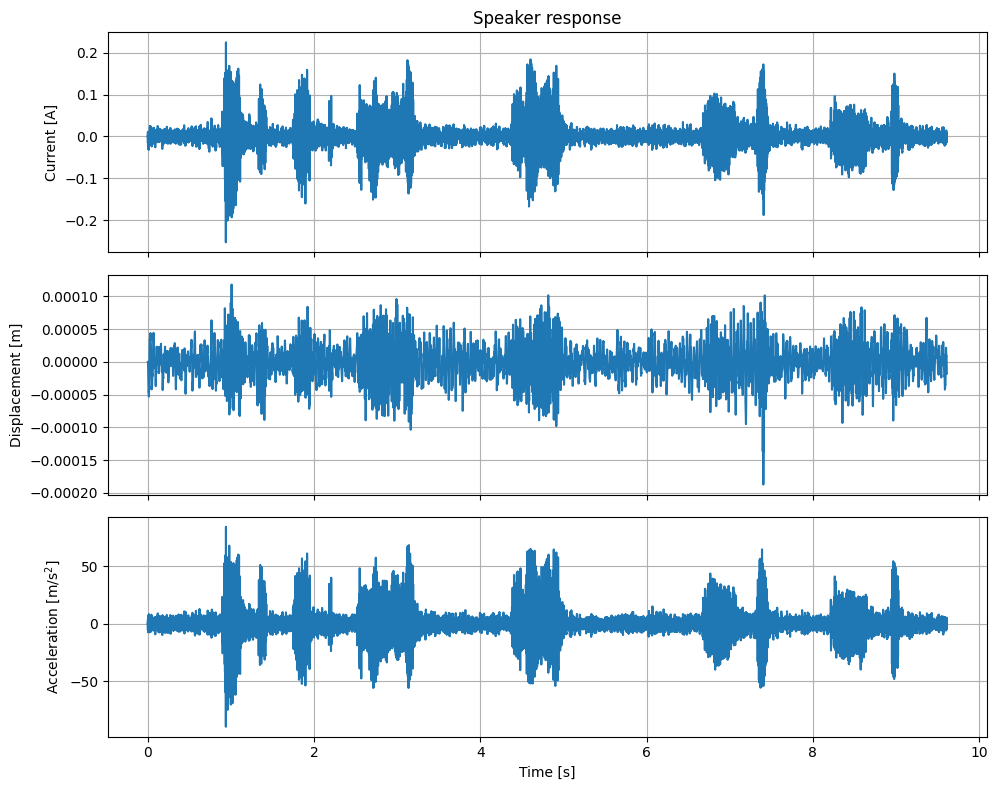
\includegraphics[width=0.88\textwidth]{fig05_nonlinear_states.png}
  \caption{Corrente, deslocamento e aceleração do modelo não linear para a gravação de voz.}
  \label{fig:naolinear}
\end{figure}

A comparação numérica é resumida na Tabela~\ref{tab:comparacao}. A corrente e a maior aceleração
permanecem praticamente iguais porque seus picos ocorrem em regiões nas quais o fator de força
ainda não sofreu redução significativa. Por outro lado, a excursão máxima cresce cerca de 54\%,
de $0{,}121$ para $0{,}187\,\mathrm{mm}$. A diferença RMS entre as acelerações é aproximadamente
9,2\% do valor RMS da aceleração linear, confirmando que a não linearidade é localizada, mas não
desprezível.

\begin{table}[H]
  \centering
  \caption{Comparação das respostas à gravação de voz.}
  \label{tab:comparacao}
  \begin{tabular}{lrr}
    \toprule
    Grandeza & Modelo linear & Modelo não linear \\
    \midrule
    Corrente máxima em módulo [A] & 0,253 & 0,253 \\
    Deslocamento máximo em módulo [mm] & 0,121 & 0,187 \\
    Aceleração máxima em módulo [m/s$^2$] & 89,3 & 89,3 \\
    Menor valor de $Bl(x)$ [N/A] & 4,95 & 0 \\
    \bottomrule
  \end{tabular}
\end{table}

A Figura~\ref{fig:comparacao-nl} evidencia que os espectros globais continuam semelhantes. A
dependência de $Bl$ com o deslocamento, entretanto, torna o sistema dependente da amplitude e
pode criar distorção, isto é, componentes espectrais que não seriam produzidas por um sistema
estritamente linear. A aceleração normalizada do segundo modelo foi salva como
\texttt{TC02-out2-nl.wav}.

\begin{figure}[H]
  \centering
  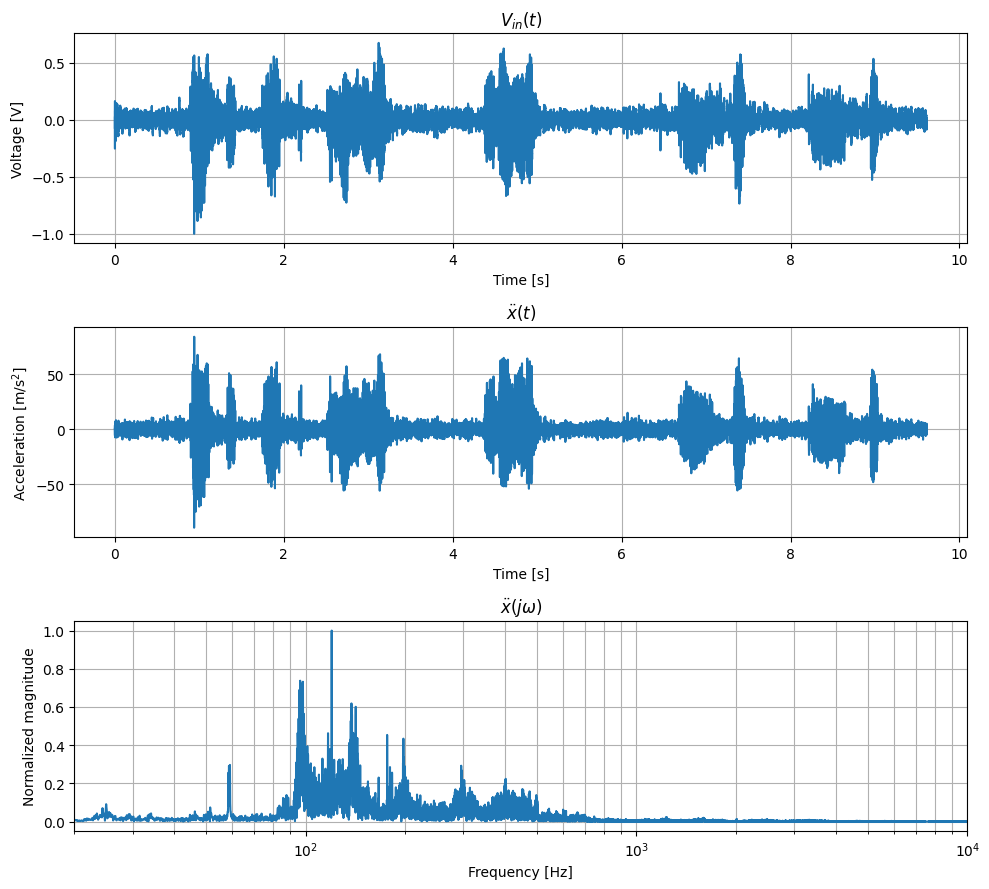
\includegraphics[width=0.86\textwidth]{fig06_nonlinear_compare.png}
  \caption{Comparação temporal entre a entrada e a aceleração, com espectro da saída não linear.}
  \label{fig:comparacao-nl}
\end{figure}

\section{Atividade 4: resposta a um sinal senoidal}

Foi empregada a entrada
\begin{equation}
  V_{in}(t)=2\sin(2\pi\,500t)\ \mathrm{V},
  \label{eq:senoide}
\end{equation}
com amplitude de $2\,\mathrm{V}$, ou $4\,\mathrm{V_{pp}}$. A frequência de $500\,\mathrm{Hz}$ está
dentro da faixa relevante para a voz humana. Como o sinal dura $9{,}61\,\mathrm{s}$, a simulação
contém cerca de 4807 períodos, muito acima do mínimo de vinte períodos solicitado.

\begin{figure}[H]
  \centering
  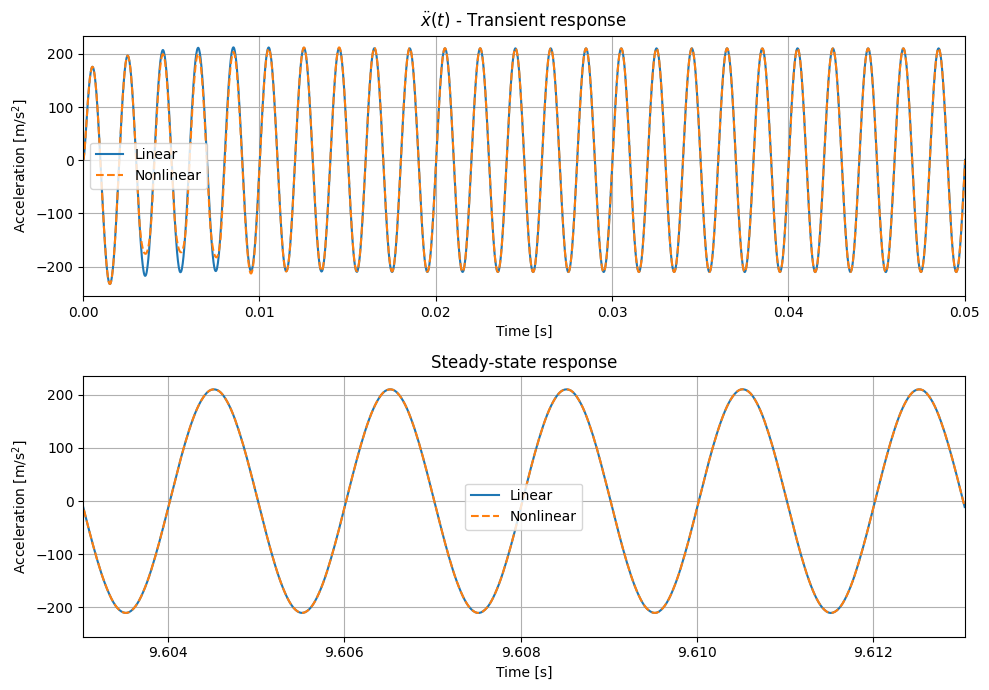
\includegraphics[width=0.89\textwidth]{fig07_sine_compare.png}
  \caption{Acelerações dos modelos linear e não linear nos regimes transitório e permanente para a entrada senoidal.}
  \label{fig:senoide}
\end{figure}

Na parte transitória da Figura~\ref{fig:senoide}, os modelos apresentam uma pequena diferença de
amplitude e fase, com diferença instantânea máxima próxima de $40{,}9\,\mathrm{m/s^2}$ nos
primeiros $50\,\mathrm{ms}$. O deslocamento transitório entra na região $|x|>x_1$, reduzindo o
fator de força a um mínimo aproximado de $3{,}92\,\mathrm{N/A}$ e alterando a troca de energia
entre os subsistemas elétrico e mecânico.

Depois que o transitório decai, as curvas tornam-se visualmente coincidentes e apresentam amplitude
de aceleração de aproximadamente $210{,}3\,\mathrm{m/s^2}$. Para uma senoide em regime permanente,
a amplitude de deslocamento pode ser estimada por
\begin{equation}
  |X|\simeq \frac{|\ddot{X}|}{(2\pi f)^2}
  =\frac{210{,}3}{(2\pi\,500)^2}
  \simeq 0{,}0213\,\mathrm{mm},
\end{equation}
valor muito inferior a $x_1=0{,}0911\,\mathrm{mm}$. Portanto, em regime permanente o fator de força
retorna a $Bl_0$ e os dois modelos são matematicamente equivalentes para essa excitação.

\section{Discussão dos resultados}

O modelo linear reproduz qualitativamente o comportamento esperado de um alto-falante: a entrada
elétrica gera corrente, a força de Laplace movimenta o cone e a suspensão limita seu deslocamento.
A resposta da aceleração preserva os principais eventos e componentes da gravação, mas modifica
suas amplitudes em função da resposta dinâmica do sistema. Isso explica por que a reprodução
sonora depende não só do sinal elétrico, mas também dos parâmetros elétricos e mecânicos do
transdutor.

A não linearidade de $Bl(x)$ é especialmente relevante nas grandes excursões. Quando $Bl$ diminui,
a corrente produz menos força e o movimento produz menos força contraeletromotriz. Essa mudança
de realimentação eletromecânica permite excursões maiores e altera localmente a aceleração. Como o
modelo coincide com o linear para $|x|\leq x_1$, sinais de pequena amplitude ou frequências que
produzem deslocamentos reduzidos não revelam diferença em regime permanente. Já a gravação de voz
contém transientes capazes de alcançar a região não linear, resultando na diferença RMS observada.

Os resultados também devem ser interpretados à luz das simplificações. Apenas $Bl$ varia com a
posição; a indutância, a rigidez e o amortecimento permanecem constantes. Não são incluídos limites
mecânicos de excursão, saturação magnética, variação térmica de $R$, modos estruturais do cone ou
propagação acústica até um microfone. Em particular, o trecho $Bl=0$ para $|x|\geq x_2$ é uma
idealização severa. Assim, os valores simulados são adequados à comparação dos modelos, mas não
constituem previsão completa de um alto-falante real.

\section{Conclusão}

O trabalho permitiu formular e simular um modelo eletromecânico de alto-falante em espaço de
estados. Para a gravação de voz, o modelo linear produziu corrente máxima de aproximadamente
$0{,}253\,\mathrm{A}$, deslocamento máximo de $0{,}121\,\mathrm{mm}$ e aceleração máxima de
$89{,}3\,\mathrm{m/s^2}$. A comparação espectral mostrou que a aceleração conserva as principais
componentes da entrada, mas é ponderada pela dinâmica do transdutor.

Ao introduzir o decaimento quadrático de $Bl(x)$, a excursão máxima aumentou para cerca de
$0{,}187\,\mathrm{mm}$ e a aceleração apresentou diferença RMS de 9,2\% em relação ao modelo
linear. Para a senoide de $500\,\mathrm{Hz}$ e $2\,\mathrm{V}$, houve diferença durante o
transitório, mas as respostas permanentes coincidiram porque o deslocamento final permaneceu abaixo
de $x_1$. Conclui-se que o modelo linear é suficiente enquanto o cone opera próximo do repouso,
mas a dependência do fator de força com a posição deve ser considerada quando transientes ou
baixas frequências produzem grandes excursões.


\end{document}
